\chapter{\IfLanguageName{dutch}{Stand van zaken}{State of the art}}%
\label{ch:stand-van-zaken}

% Tip: Begin elk hoofdstuk met een paragraaf inleiding die beschrijft hoe
% dit hoofdstuk past binnen het geheel van de bachelorproef. Geef in het
% bijzonder aan wat de link is met het vorige en volgende hoofdstuk.

% Pas na deze inleidende paragraaf komt de eerste sectiehoofding.

%-----
% Dit hoofdstuk bevat je literatuurstudie. De inhoud gaat verder op de inleiding, maar zal het onderwerp van de bachelorproef *diepgaand* uitspitten. De bedoeling is dat de lezer na lezing van dit hoofdstuk helemaal op de hoogte is van de huidige stand van zaken (state-of-the-art) in het onderzoeksdomein. Iemand die niet vertrouwd is met het onderwerp, weet nu voldoende om de rest van het verhaal te kunnen volgen, zonder dat die er nog andere informatie moet over opzoeken \autocite{Pollefliet2011}.

% Je verwijst bij elke bewering die je doet, vakterm die je introduceert, enz.\ naar je bronnen. In \LaTeX{} kan dat met het commando \texttt{$\backslash${textcite\{\}}} of \texttt{$\backslash${autocite\{\}}}. Als argument van het commando geef je de ``sleutel'' van een ``record'' in een bibliografische databank in het Bib\LaTeX{}-formaat (een tekstbestand). Als je expliciet naar de auteur verwijst in de zin (narratieve referentie), gebruik je \texttt{$\backslash${}textcite\{\}}. Soms is de auteursnaam niet expliciet een onderdeel van de zin, dan gebruik je \texttt{$\backslash${}autocite\{\}} (referentie tussen haakjes). Dit gebruik je bv.~bij een citaat, of om in het bijschrift van een overgenomen afbeelding, broncode, tabel, enz. te verwijzen naar de bron. In de volgende paragraaf een voorbeeld van elk.

% \textcite{Knuth1998} schreef een van de standaardwerken over sorteer- en zoekalgoritmen. Experten zijn het erover eens dat cloud computing een interessante opportuniteit vormen, zowel voor gebruikers als voor dienstverleners op vlak van informatietechnologie~\autocite{Creeger2009}.

% Let er ook op: het \texttt{cite}-commando voor de punt, dus binnen de zin. Je verwijst meteen naar een bron in de eerste zin die erop gebaseerd is, dus niet pas op het einde van een paragraaf.
%-----

% \lipsum[7-20]

In dit hoofdstuk wordt de literatuurstudie besproken. Het doel is om een dieper inzicht te verkrijgen in de actuele situatie binnen het onderzoeksdomein, evenals de diverse technologieën die daarmee geassocieerd worden.

\section{Spraakherkenningstechnologie}
\subsection{Introductie van spraakherkenningstechnologie}
Spraakherkenning is een technologische functionaliteit waarmee een softwareprogramma in staat is om gesproken taal te interpreteren en te verwerken in geschreven tekst. \autocite{Anusuya2009} Automatische spraakherkenning (ASR) is een specifieke vorm van spraakherkenning die het mogelijk maakt om apparaten zonder handmatige tussenkomst te besturen met spraakcommando's. Dit proces maakt menselijke tussenkomst overbodig bij het begrijpen en uitvoeren van commando's die via spraak worden gegeven. Tegenwoordig is het ook mogelijk om de input automatisch te gaan vertalen of te laten voorlezen in een gewenste taal. De opkomst van artificiële intelligentie (AI) en machine learning heeft de ontwikkeling van spraakherkenningstechnologie sterk bevorderd. Voor het gebruik van deze technologie is een microfoon nodig op het apparaat, die stemtrillingen omzet in een elektronisch signaal. Vervolgens wordt dit omgezet in een digitaal signaal dat door een spraakherkenningsprogramma kan geanalyseerd en weergegeven worden in tekst \autocite{Zwass2022}. Spraak is het gebruik van fonetische combinaties van medeklinkers en klinkers om woorden uit te drukken. Fonetiek is de studie van hoe spraak wordt geproduceerd en waargenomen, en is van essentieel belang voor de ontwikkeling van spraakherkenningstechnologie. De technologie gaat deze fonetische combinaties van spraak analyseren en omzetten in tekst \autocite{Mehrish2023}.


\subsection{De verschillende soorten spraakherkenning}
Spraakherkenning is een technologische functionaliteit waarmee een softwareprogramma in staat is om gesproken taal te interpreteren en te verwerken in geschreven tekst. \autocite{Anusuya2009} Automatische spraakherkenning (ASR) is een specifieke vorm van spraakherkenning die het mogelijk maakt om apparaten zonder handmatige tussenkomst te besturen met spraakcommando's. Dit proces maakt menselijke tussenkomst overbodig bij het begrijpen en uitvoeren van commando's die via spraak worden gegeven. Tegenwoordig is het ook mogelijk om de input automatisch te gaan vertalen of te laten voorlezen in een gewenste taal. De opkomst van artificiële intelligentie (AI) en machine learning heeft de ontwikkeling van spraakherkenningstechnologie sterk bevorderd. Voor het gebruik van deze technologie is een microfoon nodig op het apparaat, die stemtrillingen omzet in een elektronisch signaal. Vervolgens wordt dit omgezet in een digitaal signaal dat door een spraakherkenningsprogramma kan geanalyseerd en weergegeven worden in tekst \autocite{Zwass2022}. Spraak is het gebruik van fonetische combinaties van medeklinkers en klinkers om woorden uit te drukken. Fonetiek is de studie van hoe spraak wordt geproduceerd en waargenomen, en is van essentieel belang voor de ontwikkeling van spraakherkenningstechnologie. De technologie gaat deze fonetische combinaties van spraak analyseren en omzetten in tekst \autocite{Mehrish2023}.

\subsubsection{Herkenning op basis van geïsoleerde woorden}
Spraakherkenning is een technologische functionaliteit waarmee een softwareprogramma in staat is om gesproken taal te interpreteren en te verwerken in geschreven tekst. \autocite{Anusuya2009} Automatische spraakherkenning (ASR) is een specifieke vorm van spraakherkenning die het mogelijk maakt om apparaten zonder handmatige tussenkomst te besturen met spraakcommando's. Dit proces maakt menselijke tussenkomst overbodig bij het begrijpen en uitvoeren van commando's die via spraak worden gegeven. Tegenwoordig is het ook mogelijk om de input automatisch te gaan vertalen of te laten voorlezen in een gewenste taal. De opkomst van artificiële intelligentie (AI) en machine learning heeft de ontwikkeling van spraakherkenningstechnologie sterk bevorderd. Voor het gebruik van deze technologie is een microfoon nodig op het apparaat, die stemtrillingen omzet in een elektronisch signaal. Vervolgens wordt dit omgezet in een digitaal signaal dat door een spraakherkenningsprogramma kan geanalyseerd en weergegeven worden in tekst \autocite{Zwass2022}. Spraak is het gebruik van fonetische combinaties van medeklinkers en klinkers om woorden uit te drukken. Fonetiek is de studie van hoe spraak wordt geproduceerd en waargenomen, en is van essentieel belang voor de ontwikkeling van spraakherkenningstechnologie. De technologie gaat deze fonetische combinaties van spraak analyseren en omzetten in tekst \autocite{Mehrish2023}.

\subsubsection{Herkenning op basis van geconnecteerde woorden}
Deze techniek bouwt voort op de herkenning van geïsoleerde woorden en maakt het mogelijk om woorden te verbinden tot zinnen. Een beperking is echter dat er een korte pauze tussen de woorden noodzakelijk is \autocite{Maenobu1984}. Hierdoor is de snelheid van de spraakherkenning niet optimaal. De nauwkeurigheid van deze methode is vergelijkbaar met die van de herkenning van afzonderlijke woorden. De techniek vraagt echter wel een grotere rekenkracht en geheugen van het systeem \autocite{Anusuya2009}.

\subsubsection{Continue spraakherkenning}
Deze methode maakt het mogelijk om zinnen natuurlijk uit te spreken zonder dat er een pauze nodig is. Het systeem voert een doorlopende analyse en verwerking van de spraak uit, zelfs als het wordt geconfronteerd met achtergrondgeluiden \autocite{Anusuya2009}. De techniek maakt gebruik van een stappenplan zodat de spraak omgezet kan worden in tekst. In de initiële fase wordt het geluid gefilterd om ruis te minimaliseren en worden de essentiële kenmerken uit het spraakfragment gehaald. Vervolgens wordt het signaal omgezet in een reeks vectoren die de kenmerken van de spraak vertegenwoordigen, zoals het frequentie- en energieniveau. Een machine learning-model kan vervolgens deze vectoren gebruiken om de spraak te herkennen. Post-processing vormt de eindfase waarin de output verder wordt geoptimaliseerd tot een heldere, leesbare tekst \autocite{Bhatt2020}. Bij deze methode is het ook mogelijk om de tekst te gaan vertalen naar een andere taal tijdens de verwerking. De doeltreffendheid van deze benadering hangt echter in hoge mate af van zowel de kwaliteit van de trainingsdata die worden gebruikt voor het machine learning-model als van de verfijning van de ingezette algoritmes. Deze factoren spelen een cruciale rol in de bepaling van de snelheid van spraakherkenning. Dankzij deze aspecten is het mogelijk om de prestaties van verschillende modellen onderling te vergelijken en te evalueren \autocite{Bhatt2020}.

\subsubsection{Spontane spraakherkenning}
Deze techniek is de meest geavanceerde vorm van spraakherkenning. Het komt vaak voor dat ingesproken tekst niet altijd even duidelijk is, bijvoorbeeld door een hapering of een stopwoord. Spontane spraakherkenning is in staat om deze onvolkomenheden te herkennen en te verwerken waardoor de output van de spraakherkenning accurater is. Het grote verschil met continue spraakherkenning is dat daar de focus ligt op de technische uitdaging van het verwerken van gesproken taal zonder pauzes. Spontane Spraakherkenning is meer gefocust op het omgaan met de natuurlijkheid en de complexiteit van de onvoorbereide spraak waarbij er ook rekening wordt gehouden met verschillende dialecten en accenten \autocite{Vimala2012}. Het grote nadeel van deze methode is dat het een zeer complexe technologie is die veel rekenkracht en geheugen vereist waardoor de snelheid heel traag is. Dit maakt het enkel bruikbaar in specifieke toepassingen \autocite{Hori2005}. De methode maakt het ook mogelijk om tekst uit spraak te herkennen waarbij de spreker van taal kan wisselen. De methode is echter niet perfect en kan nog steeds moeilijkheden ondervinden waardoor de output niet altijd correct is \autocite{Hori2005}.



\subsection{Type spraakherkenningsmodellen gebaseerd op de spreker}
Mensen hebben verschillende manieren van spreken, zoals de snelheid, de toonhoogte, enzovoort. Hierdoor kan spraakherkenningssystemen onderverdeeld worden in twee hoofdcategorieën, namelijk spreker-afhankelijke en spreker-onafhankelijke modellen \autocite{Vimala2012}.

\subsubsection{Spreker-afhankelijke modellen}
Zoals de naam al doet vermoeden, worden deze modellen specifiek getraind en ontworpen voor één specifieke spreker. Deze aanpak is relatief eenvoudiger uit te voeren en biedt hoge nauwkeurigheid voor die specifieke spreker. Echter, het belangrijkste nadeel is de gebrek aan flexibiliteit, wat het ongeschikt maakt voor gebruik met meerdere sprekers \autocite{Vimala2012}. 

\subsubsection{Spreker-onafhankelijke modellen}
Deze modellen zijn ontworpen om spraak van verschillende sprekers te herkennen op basis van spraakpatronen en kenmerken via grote hoeveelheden trainingsdata. Het ontwikkelen van deze systemen is ingewikkeld, vergt aanzienlijk meer rekenkracht en geheugen, en bereikt over het algemeen een lagere nauwkeurigheid dan spreker-afhankelijke modellen. Het voornaamste voordeel ligt echter in de veelzijdigheid van het systeem, waardoor het toegankelijk is voor een breed publiek. Dit maakt dat het ondanks de genoemde nadelen, vaker in de praktijk worden toegepast \autocite{Vimala2012}.

\subsection{Type spraakherkenningsmodellen gebaseerd op de locatie van de verwerking}
spraakherkenningssystemen kunnen worden onderverdeeld in drie categorieën op basis van de locatie van de verwerking: geïntegreerde-, hybride- en cloud-gebaseerde spraakherkenning. Elke categorie heeft zijn eigen use-cases waarvoor het geschikt is \autocite{Leitman2020}.

\subsubsection{Geïntegreerde spraakherkenning}
Geïntegreerde spraakherkenning is een technologie die volledig lokaal op het apparaat wordt verwerkt. In deze literatuurstudie zal uitgebreider ingegaan worden op dit onderwerp, met een diepgaander inzicht en een meer gedetailleerde verkenning dan bij de andere type modellen die gebaseerd zijn op de locatie van de verwerking \autocite{Leitman2020}.

\subsubsection{Hybride spraakherkenning}
Een hybride spraakherkenningssysteem maakt gebruik van zowel lokale verwerking als verwerking in de cloud. Hierdoor kan het systeem profiteren van de voordelen van beide benaderingen. Als er een internetverbinding aanwezig is en de verwerking van de cloud snel genoeg is, gebeurd de verwerking in de cloud. Indien niet, wordt de verwerking lokaal uitgevoerd. Het nadeel van deze aanpak is dat de hardware van het apparaat krachtig genoeg moet zijn om de beslissing te maken en de verwerking te kunnen uitvoeren. Dit type spraakherkenningssysteem wordt vaak gebruikt in de software van wagens \autocite{Leitman2020}.

\subsection{Cloud-gebaseerde spraakherkenning}
Cloud-gebaseerde spraakherkenning is een technologie waarbij de verwerking van de spraak in de cloud gebeurt. De spraak die wordt opgenomen door de microfoon wordt via een Application Programming Interface (API) als aanvraag naar de cloud gestuurd. De cloud verwerkt de spraak en stuurt de output terug naar het apparaat. Het grote nadeel is dat er ten alle tijden een internetverbinding nodig is om de spraakherkenning te kunnen gebruiken \autocite{Leitman2020}.


\subsection{Type trainingsdata voor spraakherkenning}
De kwaliteit en omvang van trainingsgegevens spelen een essentiële rol in de accuraatheid van de spraakherkenningsmodellen. Deze gegevens bepalen de complexiteit en kwaliteit van de modellen, waarbij een grotere en meer gevarieerde dataset leidt tot een toename in de benodigde verwerkingstijd en geheugencapaciteit voor het trainen van de modellen. De omvang van de trainingsdata wordt uitgedrukt in aantal woorden of uren aan spraak. Naast de kwantiteit is de kwaliteit van de data ook van belang. Factoren zoals omgevingslawaai, spreekstijl, geslacht, leeftijd en spreektempo zijn heel belangrijk bij de keuze van de traingsdata \autocite{Vimala2012}.


\subsection{Hidden Markov Modellen (HMM) voor spraakherkenning}
In de jaren 70 en 80 van de vorige eeuw werden Hidden Markov Modellen (HMM) voor het eerst gebruikt voor spraakherkenning. Sindsdien zijn ze één van de meest gebruikte technieken voor spraakherkenning dankzij hun flexibele karakter. HMM's zijn statistische modellen die de waarschijnlijkheid berekenen van een specifieke reeks observaties die voortkomen uit een verborgen reeks toestanden. In spraakherkenning vertegenwoordigen de observaties, de akoestische eigenschappen van de spraak, terwijl de verborgen toestanden overeenkomen met de uitgesproken woorden. Hierdoor kunnen we de meest waarschijnlijke opeenvolging van woorden identificeren die overeenkomen met de gesproken spraak. Er zijn ook verschillende varianten van HMM's ontwikkeld die specifiek zijn afgestemd op bepaalde technologieën, waar spraakherkenningstechnologie een belangrijk voorbeeld van is. Het Hidden Semi-Markov Model (HSMM) is een voorbeeld van een variant die specifiek is ontwikkeld vanuit de ooghoek van spraakherkenning. Het biedt meer flexibiliteit dan de traditionele HMM's, wat nuttig kan zijn bij spraak die niet altijd gelijkmatig is verdeeld in tijd. In de laatste decennia zijn HMM's heel sterk verbeterd, waardoor de nauwkeurigheid van spraakherkenning mede dankzij deze techniek sterk is toegenomen. Het heeft een belangrijke rol gespeeld in het onderzoek en ontwikkeling van spraaktechnologie \autocite{Mor2020}.

\begin{figure}[H]
  \centering
  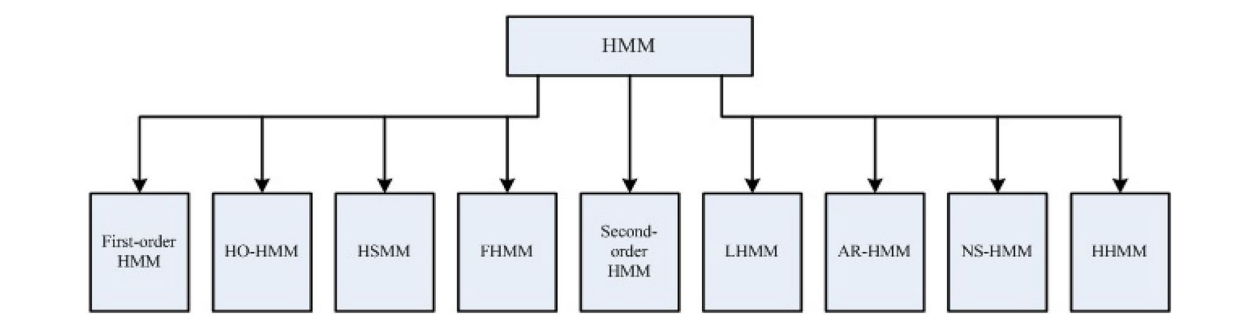
\includegraphics[scale=0.5]{Variants_HMM.png}
  \caption{Varianten van het Hidden Markov Model \autocite{Choi2020}.}
\end{figure}

\subsection{Uitdagingen in spraakherkenning}
Spraakherkenning brengen heel wat uitdagingen met zich mee. De technologie is niet perfect en heeft met bepaalde factoren te maken die de nauwkeurigheid van de spraakherkenning sterk kunnen beïnvloeden. Het moeilijkste aspect is de taaldekking voor de spraakmodellen doordat er heel veel talen bestaan en elke taal zijn eigen accenten en dialecten heeft. Een ander belangrijk spraakherkenningsprobleem is achtergrondlawaai doordat die samen met de spraak wordt opgenomen door de microfoon. Dit kan de spraakherkenning verstoren en de nauwkeurigheid verminderen. Privacy is ook een aandachtspunt bij het gebruiken van bepaalde spraakmodellen. Voor gebruik van een model kan het handig zijn om op voorhand de regels omtrent privacy door te nemen \autocite{Tate2020}.


\section{De kracht van deep learning voor spraakherkenning}
De laatste jaren heeft deep learning een grote impact gehad op de ontwikkeling van spraakherkenningstechnologie. Recent onderzoek heeft aangetoond dat spraakherkenningsmodellen die gebruik maken van deep learning technologieën, de Word Error Rate (WER) - een belangrijke indicator voor de precisie van spraakherkenning - met meer dan 50\% hebben verlaagd in vergelijking met modellen die geen deep learning toepassen \autocite{Prabhavalkar2024}. Deze technologische vooruitgang heeft geleid tot een aanzienlijke verbetering van de nauwkeurigheid van spraakherkenningssystemen. Dit heeft ertoe geleid dat spraakherkenning in de toekomst een nog grotere rol zal spelen in de ontwikkeling van nieuwe technologieën. Deep learning kan aan de hand van neurale netwerken complexe patronen in spraak herkennen die voordien nooit mogelijk waren met traditionele technieken \autocite{Prabhavalkar2024}.

\subsection{Artificiële intelligentie, machine learning, deep learning en neurale netwerken: wat is het verschil?}
Artificiële intelligentie (AI) is een overkoepelende term die zich bezig houdt met het creëren van intelligentie in machines. Binnen het domein van AI valt Machine learning dat zich focust op het ontwikkelen van algoritmes waarmee computers kunnen leren van ingevoerde data en patronen. Deep learning is een verzamelnaam voor een reeks van technieken voor zelfsturende machine learning, waarbij algoritmes zichzelf kunnen aanpassen op basis van externe data. Neurale netwerken zijn algoritmen die patronen kunnen herkennen in data. Deep learning maakt gebruik van neurale netwerken om op basis van deze patronen voorspellingen te maken en zichzelf te verbeteren. Deze termen worden heel vaak door elkaar gebruikt, maar het is belangrijk om te weten dat ze niet hetzelfde zijn. Door deze technieken heeft datawetenschap een enorme groei gekend \autocite{Choi2020}

\begin{figure}[H]
  \centering
  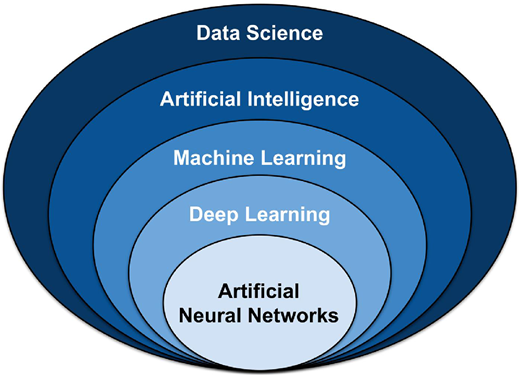
\includegraphics[scale=2]{Intro_ML_NeuralNetw_DeepL.png}
  \caption{Datawetenschap technieken \autocite{Choi2020}.}
\end{figure}

\subsection{Gebruik van deep learning voor spraakherkenning}
Door het gebruik van meerdere verwerkingslagen in spraakherkenning, is het mogelijk om complexe patronen in spraak te herkennen. Deze patronen worden gekend doordat er gebruik wordt gemaakt van neurale netwerken. Er zijn verschillende soorten neurale netwerken die elk hun eigen voordelen en doeleinden hebben. De meest gebruikte netwerken in spraakherkenning zijn recurrente neurale netwerken (RNN) en convolutionele neurale netwerken (CNN). Deze technieken hebben geleid tot enorme verbeteringen in (automatische) spraakherkenning, tekst-naar-spraaktechnologie en emotieherkenning in spraak. Het heeft ook aanzienlijke vooruitgang geboekt in de ontwikkeling van diverse uitdagingen in spraakherkenning zoals het omgaan met luidruchtige omgevingen, verschillende accenten en dialecten, enzovoort \autocite{Mehrish2023}.

\subsubsection{Recurrente neurale netwerken (RNN)}
Door het dynamische karakter van spraak zijn RNN's zijn niet meer weg te denken uit de wereld van spraakherkenningstechnologie die gebruik maakt van neurale netwerken. RNN's kunnen sequentiepatronen modelleren die anders moeilijk vast te leggen zijn met andere neurale architecturen \autocite{Mehrish2023}. Meer specifiek zijn ze ontworpen om tijdreekssignalen te modelleren en afhankelijkheden op lange en korte termijn tussen verschillende tijdsmomenten te identificeren \autocite{Papastratis2021}. Het voordeel van deze neurale techniek is dat het in staat is om de output te voorspellen op basis van de vorige input, wat de volgende input zal zijn. Hierdoor kan de context van spraak beter begrepen en verwerkt worden \autocite{Mehrish2023}. Daarbij is ook een nadeel aan verbonden, namelijk dat enkel de vorige input wordt gebruikt wat kan zorgen voor onnauwkeurigheden in de voorspelling. In het algemeen functioneren RNN's heel goed waardoor ze wel een belangrijke rol spelen \autocite{Papastratis2021}. RNN's worden vaak in combinatie gebruikt met Hidden Markov Modellen (HMM) voor spraakherkenning. Het nadeel van de hybride aanpak is dat HMM's specifieke kennis vereist om het model te kunnen gebruiken. Dit kan ervoor zorgen dat het systeem fouten kan maken bij het herkennen van spraak omdat de RNN's niet optimaal de patronen kunnen herkennen \autocite{Mehrish2023}.

\subsubsection{Convolutionele neurale netwerken (CNN)}
Deze techniek is een gespecialiseerde klasse van de neurale architectuur. Het concept van convolutionele neurale netwerken is aanvankelijk ontwikkeld voor het verwerken van visuele gegevens. Deze technologie werkt door kleine delen van de invoergegevens te analyseren, waardoor het probeert te identificeren wat er in die gegevens aanwezig is. Deze patronen worden vervolgens gebruikt om de gegevens te classificeren. Bij spraakherkenning wordt deze techniek vooral gebruikt om patronen te vinden tussen de verschillen van sprekers en de manier van praten. Hierdoor kunnen deze patronen gebruikt worden om nauwkeuriger de spraak te herkennen. Het grote voordeel van CNN's is dat ze minder gevoelig zijn voor ruis en achtergrondgeluiden \autocite{Mehrish2023}.


\section{Geïntegreerde spraakherkenning}
Spraakherkenning heeft de laatste jaren een enorme groei gekend. Technisch gezien zit spraakherkenningstechnologie al in een gevorderd stadium. Deze oplossing wordt gebruikt in verschillende toepassingen, in verschillende sectoren en is momenteel vooral gericht op desktop computers. Hierdoor is de uitdaging in de technologie om spraakherkenning te integreren op apparaten met beperkte middelen zoals smartphones, tablets, enzovoort \autocite{Tan2008}. Deze apparaten hebben beperkte rekenkracht en geheugen, lage batterijduur en vaak geen internetverbinding. Een smartphone is niet meer weg te denken uit onze samenleving door de multifunctionaliteit en draagbaarheid van het toestel. Bij het ontwikkelen van geïntegreerde spraakherkenningstechnologie moet alle verwerking op het apparaat zelf gebeuren en mag er geen gebruik gemaakt worden van externe servers. Hierdoor moet er rekening gehouden worden met de hardware, die bestaat uit de processor (CPU), het geheugen (RAM) en nog andere componenten. De spraak wordt opgenomen via de microfoon in het toestel en vervolgens verwerkt met behulp van de rekenkracht van de processor en het tijdelijke geheugen om spraakherkenning mogelijk te maken. De bedoeling is dat de output dan in real-time wordt weergegeven op het scherm van het apparaat \autocite{Yehui2016}.

\subsection{Integratie van geïntegreerde spraakherkenning in Android \\smartphones}
Android is een besturingssysteem voor smarthpones dat ontwikkeld is door Google. Het besturingssysteem is open-source en is ontwikkeld op basis van de Linux-kernel. Momenteel is Android het meest gebruikte besturingssysteem voor smartphones en tablets. Android biedt een breed scala aan functionaliteiten en mogelijkheden voor ontwikkelaars om applicaties te ontwikkelen voor het besturingssysteem \autocite{Karch2021}. De integratie met geïntegreerde spraakherkenningstechnologieën in smarthpones met Android als besturingssysteem gebeurt vaak via een Software Development Kit (SDK) die ontwikkelaars kunnen gebruiken om spraakherkenning toe te voegen aan hun applicaties. Een SDK bevat een reeks van tools, bibliotheken en documentatie waarmee ontwikkelaars technologische functionaliteiten kunnen integreren in hun applicaties, zonder zelf de onderliggende technologie te hoeven ontwikkelen. Dit maakt het ontwikkelproces veel eenvoudiger en sneller. De SDK's zijn vaak beschikbaar voor verschillende programmeertalen en besturingssystemen, waardoor ze breed inzetbaar zijn. SDK's kunnen gebruik maken van een Application Programming Interface (API) die zorgt voor de communicatie tussen de technologie in de applicatie en een externe server. Doordat hier geen gebruik van kan gemaakt worden voor een geïntegreerde oplossing, moet de SDK de mogelijkheid hebben om de spraakherkenning volledig lokaal te verwerken \autocite{Fitzgerald2023}. 

% \newline \newline

% TO DO:
% Er wordt verder onderzoek gedaan naar de verschillende Embedded Speech-To-Text technologieën die beschikbaar zijn voor Android smartphones. Deze worden kort besproken in de volgende alinea's. Ik denk dat ik dit kan beschrijven in 1-2 pagina's.

\section{Geïntegreerde Speech-To-Text modellen voor Android smartphones}
Op dit moment zijn er diverse spraakherkenningstechnologieën beschikbaar die ontwikkelaars kunnen integreren in hun applicaties. Alle grote multinationals, waaronder Google, Microsoft, Amazon, en IBM, beschikken over hun eigen modellen voor spraakherkenning. Het grote nadeel is dat deze modellen vaak gebruik maken van cloud-gebaseerde verwerking, waardoor ze niet geschikt zijn voor een geïntegreerde oplossing. De achterliggende reden is de commercialisering van applicaties met spraakherkenning en verwerking in de cloud die kosten voor de ontwikkelaar met zich meebrengt, wat resulteert in winstgevendheid voor de bedrijven die deze technologieën aanbieden. Spraakmodellen die verwerkt worden in de cloud zijn ook vaak beter in het herkennen van spraak doordat de cloud meer rekenkracht heeft en beter getraind is voor verwerking. De modellen die wel lokaal spraak kunnen verwerken, komen vaak van kleinere bedrijven die een open-source oplossing aanbieden. Deze bedrijven rekenen vaak op ontwikkelaars die helpen bij het verder ontwikkelen van het model. Het grote nadeel is dat deze modellen vaak minder nauwkeurig zijn in het herkennen van spraak doordat ze minder goed getraind zijn voor verwerking. Hierdoor zijn er ook maar een beperkt aantal modellen beschikbaar die lokaal spraak kunnen verwerken. In de volgende alinea's worden de modellen die geïntegreerd kunnen worden in Android smartphones kort besproken \autocite{Richards2024}.

% \subsection{Vosk}
% Vosk is een open-source spraakherkenningstechnologie die een toolkit aanbiedt voor het ontwikkelen van spraakherkenning in applicaties. Het maakt gebruik van algoritmes van Kaldi, een toolkit voor spraakherkenning die ontwikkeld is in de programmeertaal C++, maar is geoptimaliseerd voor ontwikkelaars die spraakherkenning willen integreren in hun applicaties. Het model kan als geïntegreerde oplossing gebruikt worden in Android smartphones. Het ondersteund meer dan 20 talen en dialecten waaronder Engels, Frans en Nederlands. Het biedt ook een API aan waarmee ontwikkelaars de keuze krijgen om de spraakherkenning lokaal of in de cloud te verwerken. Deze compacte oplossing vereist slechts 50Mb aan opslagruimte en gebruikt ongeveer 300Mb aan geheugen tijdens uitvoering. Naast de spraakherkenning biedt Vosk ook de mogelijkheid om aan spreker identificatie te doen \autocite{HafizMuhammad2022}.

\subsection{Whisper}
Whisper is een open-source spraakherkenningstechnologie die ontwikkeld is door OpenAI. Dit bedrijf is bekend voor zijn ontwikkeling van artificiële intelligentie en machine learning technologieën. Whisper heeft verschillende spraakmodellen ter beschikking die ontwikkelaars kunnen integreren in applicaties. De modellen zijn geschikt voor lokale verwerking en worden ondersteund op Android-smartphones. De taalondersteuning is verschillend per model \autocite{Griffiths2023}. De modellen zijn getraind op 680 000 uur aan spraakdata dat afkomstig is van het web. Eén derde hiervan is niet-Engelse spraakdata, wat de modellen beter maakt in het herkennen van spraak in verschillende talen \autocite{OpenAI2023}. 
 Whisper biedt ook de mogelijkheid om spraakherkenning in real-time te verwerken via een API \autocite{Griffiths2023}.

\subsection{Microsoft Embedded Speech-To-Text}
Dit is een model die ontwikkeld is door Microsoft, één van de grootste technologiebedrijven ter wereld. Het is een model dat geïntegreerde spraakherkenning mogelijk maakt via een SDK. Het model kan ontwikkeld worden voor Android smartphones. Het biedt wel geen taalondersteuning voor het Nederlands, maar wel voor het Engels en Frans. Het model is beschikbaar voor hybride verwerking als ook voor lokale verwerking \autocite{Shah2023}.

\subsection{Mozilla DeepSpeech}
Mozilla DeepSpeech is een open-source spraakherkenningstechnologie die is ontwikkeld door Mozilla, de organisatie achter de welbekende browser Firefox. Het bedrijf heeft de laatste jaren sterk bijgedragen aan de ontwikkeling van open-source spraakherkenningstechnologieën. Op dit moment ondersteunt het model alleen de Engelse taal. Het model is beschikbaar voor lokale verwerking en kan geïntegreerd worden in Android smartphones. Het maakt gebruik van Google Tensorflow, een platform die ontwikkelaars kunnen gebruiken om machine learning modellen te ontwikkelen. Dit maakt het model heel flexibel en eenvoudig te integreren in applicaties \autocite{Tang2021}.

\subsection{Picovoice Cheetah}
Picovoice Cheetah is een geïntegreerde spraakherkenningsmodel die ontwikkeld is door Picovoice, een bedrijf dat gespecialiseerd is in spraakherkenning. Het model gebruikt het deep learning model van Picovoice. Het is offline beschikbaar en kan geïntegreerd worden in Android smartphones. Het model neemt 71.3Mb aan opslagruimte in beslag, wat relatief weinig is voor een geïntegreerde oplossing. Momenteel biedt het model enkel ondersteuning voor de Engelse taal \autocite{Halfacree2022}.